\documentclass[11pt,a4paper]{article}

\usepackage[utf8]{inputenc}
\usepackage[T1]{fontenc}
\usepackage{lmodern}
\usepackage[margin=2.4cm]{geometry}
\usepackage{amsmath,amssymb}
\usepackage{booktabs}
\usepackage{graphicx}
\usepackage{float}
\usepackage{array}
\usepackage{multirow}
\usepackage{tabularx}
\usepackage{xcolor}
\usepackage{caption}
\usepackage{subcaption}
\usepackage{enumitem}
\usepackage[hidelinks]{hyperref}

\captionsetup{font=small,labelfont=bf}
\setlist{itemsep=2pt,topsep=4pt}
\newcommand{\RMSE}{\mathrm{RMSE}}
\newcommand{\GEH}{\mathrm{GEH}}
\newcommand{\pass}{\textcolor{green!45!black}{yes}}
\newcommand{\fail}{\textcolor{red!70!black}{no}}

\title{Calibration and Alternative Designs of the Kungsgatan and Slottsgatan Vissim Model\\[2pt]
\large Automated batch simulation, Gaussian-process surrogates, validation and scenario analysis}
\author{Muhammad Noman Tabassum\\ Infra Informatics PhD course, Simulation module (Vissim lab)}
\date{October 2026}

\begin{document}
\maketitle

\begin{abstract}
This report documents the calibration of the course Vissim model of the signalised intersection
Kungsgatan and Slottsgatan in Norrk\"oping against mean speeds and accelerations measured on ten
weekday mornings at twelve locations. Instead of the manual one-parameter-at-a-time procedure,
the model was driven automatically from Python through the Vissim COM interface. In total about
1\,860 simulation runs were performed in three calibration phases. Each phase consisted of a
space-filling Latin hypercube design, a Gaussian-process (GP) surrogate model for every
measured quantity, a global sensitivity analysis based on Sobol indices, a constrained
optimisation on the surrogate, a local refinement design and an independent validation with new
random seeds. Phase~1 calibrated on speeds only and reduced the speed RMSE from 4.53 to
1.34~km/h, but did so by unrealistically gentle braking that destroyed the acceleration profile.
Phase~2 calibrated speeds and accelerations jointly with direction-specific desired speeds and
is the recommended calibrated model: the speed RMSE is halved to 2.01~km/h, the acceleration RMSE
stays at the level of the original model (0.13~m/s$^2$), all four bicycle locations and the
approaches L6 to L8 pass the course $t$-test, the demand is fully served (maximum GEH 0.68) and the
result holds on odd and even field days separately. Phase~3 added more freedom (shape of the
acceleration function, separate right-turn speeds) and an objective that maximises the number of
passed $t$-tests; it confirmed that the remaining discrepancies are structural rather than a
matter of parameter values. The calibrated model was then used to evaluate the three alternative
designs of the lab with 20 paired replications each. An actuated signal controller reduces the
average delay by 26\,\% (21.3 to 15.7~s per vehicle) by giving the green time of the lightly loaded
side road to the near-saturated main road. A 10-minute redistribution of the demand caused by an
incident creates temporary queues on Slottsgatan that dissolve within the next interval. An increase
of the bicycle demand to 800 per direction reduces the car throughput on Kungsgatan by 7\,\% through
the conflict with right-turning vehicles and doubles the number of stops.
\end{abstract}

\tableofcontents
\newpage

%=====================================================================
\section{Introduction and objectives}
%=====================================================================

The purpose of the exercise is to calibrate a microscopic traffic simulation model so that it
reproduces measured traffic behaviour at a signalised intersection, and to use the calibrated model
as the baseline for the analysis of alternative designs. The field data consist of mean speeds at
twelve locations (eight for motorised traffic, four on the cycle tracks) and mean accelerations at
the eight motorised locations, observed on ten weekday mornings under the current fixed-time signal
control and fixed traffic demand.

The lab instructions suggest calibrating by adjusting one parameter at a time, for example the
average standstill distance, the additive and multiplicative factors of the safety distance, the
desired speed distributions and the desired acceleration and deceleration functions. With roughly
fifteen candidate parameters that interact non-linearly through queues, capacity and signal timing,
a one-at-a-time search covers only a tiny part of the parameter space and gives no information
about interactions. The objectives of this work were therefore:
\begin{enumerate}
  \item to analyse the model in detail and identify every model element that can influence the
        measured speeds and accelerations;
  \item to automate the generation, simulation and evaluation of model variants;
  \item to run enough simulations of systematically varied parameter combinations to train a
        machine-learning surrogate model of the simulator;
  \item to find optimal parameter values on the surrogate under explicit realism constraints;
  \item to validate the result with independent random seeds and the statistical tests of the
        course, and to report how many replications are required.
\end{enumerate}

%=====================================================================
\section{The simulation model}
%=====================================================================

\subsection{Network, demand and signal control}

The model (\texttt{Vissim\_lab.inpx}, PTV Vissim 2026, Thesis licence) contains one four-armed
intersection (Figure~\ref{fig:network}). Each approach has one lane with a short left-turn pocket.
Vehicles are generated by four vehicle inputs and distributed by static routing decisions;
pedestrians and bicycles have their own inputs on footpaths and cycle tracks. Table~\ref{tab:demand}
summarises the motorised demand.

\begin{table}[H]
\centering
\caption{Motorised demand of the model (vehicles per hour, constant over the period). The vehicle
composition is 95\,\% cars and 5\,\% heavy goods vehicles (HGV).}
\label{tab:demand}
\small
\begin{tabular}{llrl}
\toprule
\textbf{Input} & \textbf{Approach (link)} & \textbf{Volume} & \textbf{Left / straight / right}\\
\midrule
1  & Kungsgatan from the north, southbound (4) & 660  & 0.06 / 0.79 / 0.15\\
3  & Kungsgatan from the south, northbound (2) & 1040 & 0.08 / 0.75 / 0.17\\
4  & Slottsgatan from the east, westbound (5)   & 240  & 0.50 / 0.08 / 0.42\\
11 & Slottsgatan from the west, eastbound (11)  & 210  & 0.29 / 0.14 / 0.57\\
14, 15 & Cycle tracks along Kungsgatan        & 100 each & straight only\\
\bottomrule
\end{tabular}
\end{table}

The signal controller is a stage-based fixed-time controller (program~1, cycle time 90~s). Stage~1
serves Kungsgatan and its bicycles, stage~2 serves Slottsgatan. Decoding the controller data stored
in the network file gives an effective green time of about 48~s for Kungsgatan and 38~s for
Slottsgatan, with intergreen periods of 11~s and 14~s. With a saturation flow of about 1\,900~veh/h
the single northbound lane on Kungsgatan has a capacity of roughly
$1900 \cdot 48/90 \approx 1010$~veh/h, while its straight and right-turning demand passing the
stop line is 957~veh/h. This approach therefore operates at a degree of saturation of about 0.95,
which makes it very sensitive to every parameter that changes the saturation flow.

\subsection{Measurement locations}

The twelve measurement locations L1 to L12 are the Vissim data collection measurements 1 to 12.
Their exact positions were extracted from the network file (Table~\ref{tab:locations}). The
location of a point relative to the stop line determines what it measures: exit points (L2, L3,
L5, L6) are dominated by acceleration towards the desired speed, approach points (L1, L4, L8) by
deceleration and queueing, and L7, which lies 2.2~m \emph{after} the southbound stop line,
measures the discharge of the queue. Left-turning vehicles leave the main lane into the turn
pocket upstream of L1, L4, L7 and L8; at L1 and L8 the observed stream consists mostly of
right-turners (84\,\% and 67\,\%).

\begin{figure}[H]
\centering
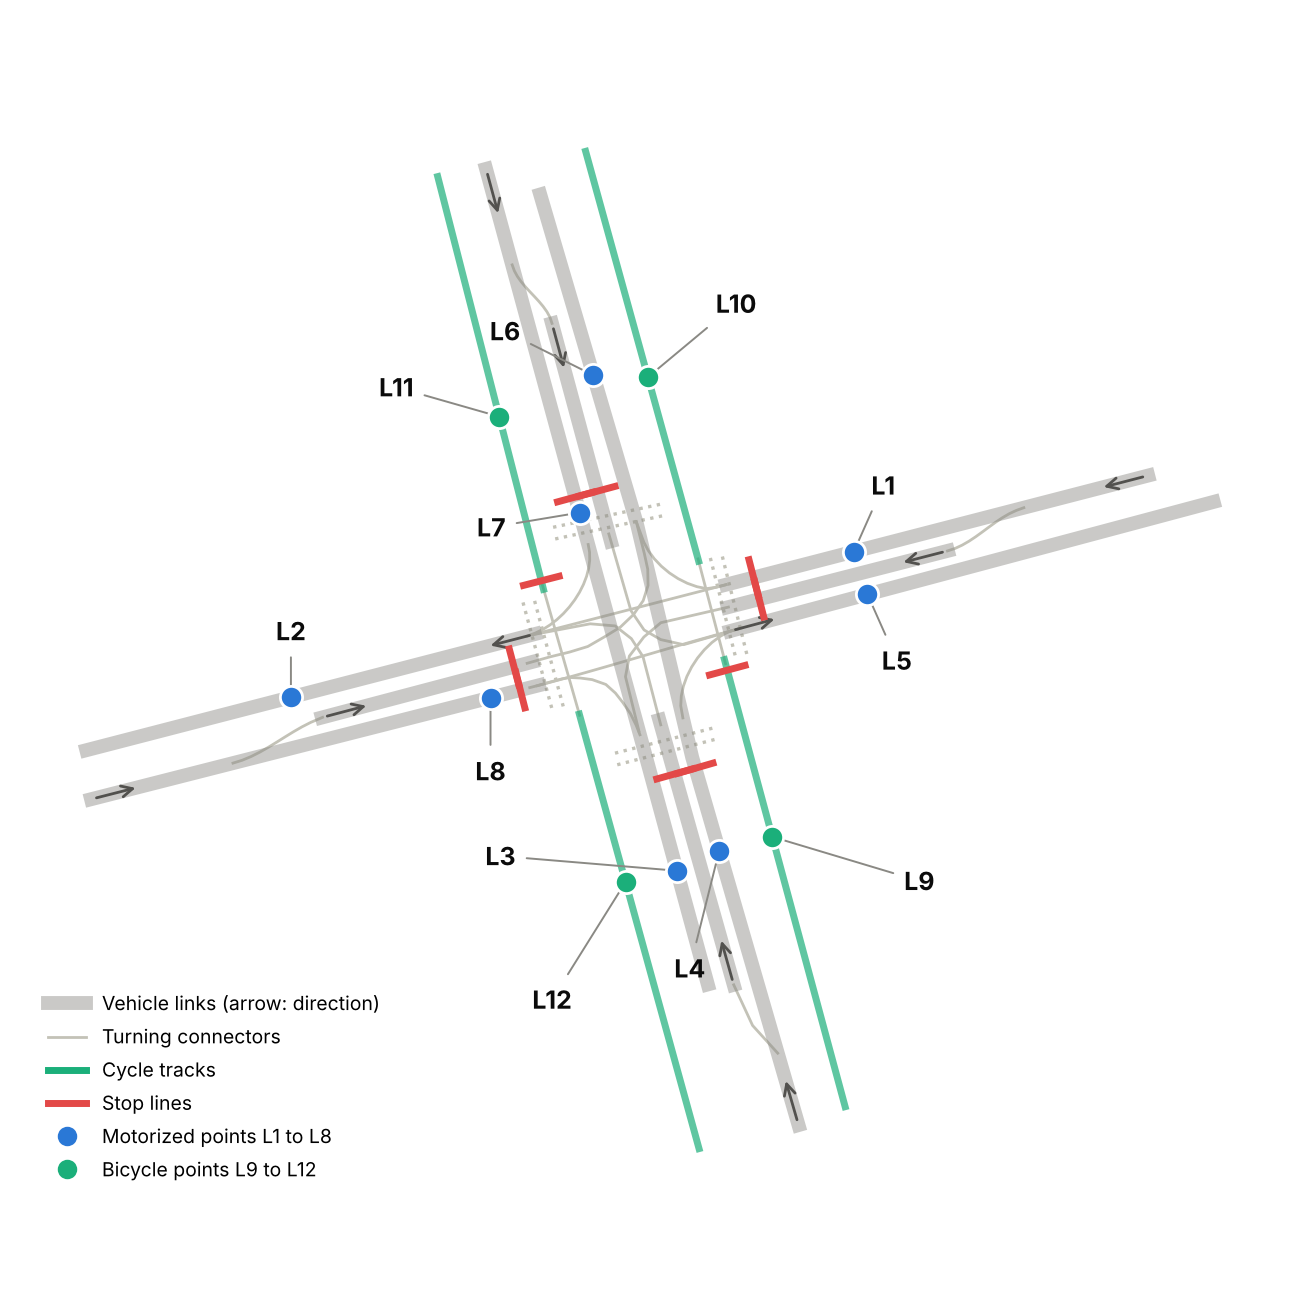
\includegraphics[width=0.78\textwidth]{fig_network.png}
\caption{Vissim network with links, turning connectors, stop lines and the twelve data collection
points. Plotted from the coordinates in \texttt{Vissim\_lab.inpx}.}
\label{fig:network}
\end{figure}

\begin{table}[H]
\centering
\caption{Measurement locations, expected hourly flow (input volume times route share) and field
statistics over the ten mornings (mean and day-to-day standard deviation).}
\label{tab:locations}
\footnotesize
\setlength{\tabcolsep}{4pt}
\begin{tabular}{lllrrrrr}
\toprule
& & & \textbf{Flow} & \multicolumn{2}{c}{\textbf{Speed [km/h]}} & \multicolumn{2}{c}{\textbf{Acc. [m/s$^2$]}}\\
\cmidrule(lr){5-6}\cmidrule(lr){7-8}
\textbf{Loc.} & \textbf{Name} & \textbf{Position} & \textbf{[veh/h]} & \textbf{mean} & \textbf{s.d.} & \textbf{mean} & \textbf{s.d.}\\
\midrule
L1  & Slottsgatan East in   & 14.0 m before stop line & 120  & 17.46 & 4.655 & $-1.787$ & 0.102\\
L2  & Slottsgatan West out  & 34 m after junction     & 142  & 48.71 & 0.688 & 0.763 & 0.083\\
L3  & Kungsgatan South out  & 52.6 m after stop line  & 702  & 49.06 & 0.335 & 0.505 & 0.035\\
L4  & Kungsgatan South in   & 11.7 m before stop line & 957  & 27.00 & 1.629 & $-0.214$ & 0.080\\
L5  & Slottsgatan East out  & 19 m after junction     & 305  & 40.20 & 0.485 & 1.600 & 0.035\\
L6  & Kungsgatan North out  & 55.3 m after stop line  & 1001 & 46.80 & 0.444 & 0.724 & 0.032\\
L7  & Kungsgatan North in   & 2.1 m \emph{after} stop line & 561 & 34.41 & 1.414 & 0.966 & 0.069\\
L8  & Slottsgatan West in   & 4.1 m before stop line  & 90   & 19.05 & 1.963 & $-0.710$ & 0.258\\
\midrule
L9  & Kungsgatan South in (bike)  & cycle track & 100 & 18.07 & 0.547 & & \\
L10 & Kungsgatan North out (bike) & cycle track & 100 & 17.70 & 0.574 & & \\
L11 & Kungsgatan North in (bike)  & cycle track & 100 & 18.07 & 0.316 & & \\
L12 & Kungsgatan South out (bike) & cycle track & 100 & 17.77 & 0.331 & & \\
\bottomrule
\end{tabular}
\end{table}

The day-to-day variability differs by more than an order of magnitude between locations:
the standard deviation of the mean speed is 4.66~km/h at L1 but 0.34~km/h at L3. This
heterogeneity turned out to be decisive for the choice of the calibration objective
(Section~\ref{sec:phase3}).

\subsection{Model inventory: what can influence speeds and accelerations}

A complete inventory of the behavioural model elements was made from the network file:
\begin{itemize}
  \item \textbf{Car following.} All motorised links use driving behaviour~1, Urban (motorised),
  Wiedemann~74 with $a_x = 2.0$~m, $b_{x,\mathrm{add}} = 2.0$ and $b_{x,\mathrm{mult}} = 3.0$ and a
  safety-distance reduction factor of 0.6 close to stop lines. Cycle tracks use Wiedemann~99
  (driving behaviour~5), footpaths use no interaction.
  \item \textbf{Desired speeds.} Composition~1 (Default) assigns the distribution ``50'', uniform
  between 48 and 58~km/h, to cars and HGVs of all four inputs. Compositions~4 (CarKungsgatan) and
  5 (CarSlottsgatan) exist but are unused. Bicycles use $U(12,15)$ (80\,\%) and e-bikes $U(15,20)$
  (20\,\%) km/h.
  \item \textbf{Acceleration and deceleration.} Cars and HGVs have speed-dependent desired and
  maximum acceleration and deceleration functions; the desired deceleration of cars is
  $-2.75$~m/s$^2$.
  \item \textbf{Turning speeds.} Reduced-speed areas on the right-turn connectors (areas 1, 4, 5, 9)
  use $U(20,25)$~km/h for cars and $U(25,30)$~km/h for HGVs, but area~9 has these two swapped.
  Three of the four left-turn areas (6, 7, 8) contain no speed at all, the fourth (area~10) uses
  $U(25,30)$ and $U(20,25)$~km/h.
  \item \textbf{Conflict areas.} 91 conflict areas, all with default gaps (front and rear gap
  0.5~s, safety distance factor 1.5). Right-turning vehicles yield to pedestrians and cyclists.
  \item \textbf{Evaluation settings.} The original simulation period was 1\,800~s with data
  collection from $t=0$, i.e.\ on an initially empty network without warm-up.
\end{itemize}

%=====================================================================
\section{Methodology}
%=====================================================================

\subsection{Automation of Vissim}

A Python tool chain (Python 3.14, \texttt{pywin32}, \texttt{numpy}, \texttt{pandas},
\texttt{scipy}, \texttt{scikit-learn}) was developed to run the complete calibration without manual
interaction. It consists of five modules:
\begin{description}
  \item[\texttt{build\_net.py}] writes a model variant for a given parameter vector by editing the
  XML of the original \texttt{.inpx}: driving-behaviour attributes, new uniform desired-speed
  distributions, vehicle compositions and their assignment to vehicle inputs, scaling of the
  acceleration and deceleration functions, reduced-speed areas, conflict-area gaps, simulation
  period and evaluation interval. Every speed parameter becomes a real Vissim distribution
  $U(c-w, c+w)$, so continuous parameter values are valid model inputs.
  \item[\texttt{design.py}] creates Latin hypercube designs and refinement designs.
  \item[\texttt{run\_vissim.py}] stages each variant in a temporary folder, loads it through the
  COM interface, sets the number of runs and the random seeds, runs the simulation in quick mode,
  reads speed, acceleration and vehicle counts of every data collection measurement and every
  replication, parses the Vissim error files for vehicle inputs that could not be completed, and
  appends the results to a CSV file. Interrupted batches resume automatically.
  \item[\texttt{analyse.py}] computes all statistics, trains the surrogates, performs the
  sensitivity analysis and the optimisation, writes the validation design and the final report.
  \item[\texttt{run\_pipeline.py}] executes screening, refinement and validation in sequence.
\end{description}

Two practical obstacles were solved during development. First, the original network belonged to
a Vissim scenario-management project; such a file can only be loaded next to its project
database and cannot be simulated outside the ``Edit scenario'' mode. Every generated variant is
therefore written as a stand-alone network. Second, the result attributes of the COM interface
were verified with a smoke test before the large batches. The original \texttt{Vissim\_lab.inpx}
was never modified.

\subsection{Common settings of all simulations}

\begin{itemize}
  \item Fixed-time controller~1, program~1; demand and routes unchanged.
  \item Simulation period 2\,400~s: 600~s warm-up followed by 1\,800~s of data collection
        (one aggregation interval). The warm-up removes the bias of an initially empty network.
  \item Calibration runs: 3 replications per configuration with common random numbers
        (seed 42, increment 1), so that differences between configurations are not masked by
        random variation.
  \item Validation runs: 10 replications with independent seeds (seed 1001, increment 7).
  \item Simulation resolution 10 time steps per second (unchanged).
\end{itemize}
One configuration with three replications took about 21~s in quick mode.

\subsection{Statistical comparison with the field data}

For every location the course two-sample $t$-test with pooled variance was applied,
\begin{equation}
T = \frac{\bar x - \bar y}{\sqrt{s_p^2\left(\frac{1}{n_x}+\frac{1}{n_y}\right)}},\qquad
s_p^2 = \frac{(n_y-1)s_y^2 + (n_x-1)s_x^2}{n_x+n_y-2},
\end{equation}
with $\bar y, s_y$ the field mean and standard deviation over $n_y = 10$ days and $\bar x, s_x$
the simulated mean and standard deviation over $n_x$ replications. $H_0$ (equal means) is kept if
$|T| < t_{0.975,\,n_x+n_y-2}$, which is 2.101 for the validation with $n_x = 10$. The required
number of replications follows the course formula
\begin{equation}
n = \left(\frac{t_{0.975,\,n_x-1}\, s_x}{\varepsilon\, \bar x}\right)^2, \qquad \varepsilon = 0.05 .
\end{equation}
In addition, the root mean square error over locations, $\RMSE = \sqrt{\frac{1}{m}\sum_i (\bar x_i-\bar y_i)^2}$,
was computed separately for speeds ($m=12$) and accelerations ($m=8$).

\subsection{Realism constraints: demand must be served}

Larger safety distances lower the saturation flow. On the near-saturated northbound approach this
creates a queue that grows back to the network entry, vehicles can no longer be generated, and
the simulated flow at L4 falls below the demand. In such a model the approach speed at L4
decreases, which superficially improves the fit, but for the wrong reason. Two constraints were
therefore imposed on every candidate:
\begin{align}
\GEH_i &= \sqrt{\frac{2 (q_i^{\mathrm{sim}}-q_i^{\mathrm{exp}})^2}{q_i^{\mathrm{sim}}+q_i^{\mathrm{exp}}}} \le 5, \quad i = 1,\dots,8,\\
q_4^{\mathrm{sim}} &\ge 0.97\, q_4^{\mathrm{orig}},
\end{align}
where $q_i^{\mathrm{exp}}$ is the expected hourly flow of Table~\ref{tab:locations} and
$q_4^{\mathrm{orig}}$ is the flow at L4 in the original model. The second constraint is relative,
because even the uncongested original model counts slightly less than the theoretical demand at L4
(detector position, stochastic arrivals). On the surrogate a safety margin was used
($\GEH \le 4$, served flow one percentage point above the threshold).

\subsection{Experimental design}

Each phase started with a Latin hypercube sample (centred-discrepancy optimised) over the parameter
box, plus the original model and the parameterised baseline as references. After the first
surrogate optimisation a refinement design of 40 points was drawn in a box of $\pm 25\,\%$ of the
range around the surrogate optimum, together with the optimum itself, and the surrogate was retrained
on all data.

\subsection{Gaussian-process surrogate}

For each output (twelve speeds, eight flows, eight accelerations) an independent GP regression
model was fitted on the configuration means, with inputs scaled to $[0,1]^d$. The kernel is
\begin{equation}
k(\mathbf u,\mathbf u') = \sigma_f^2\, k_{\mathrm{Mat\acute ern},\,\nu=5/2}\!\left(\mathbf u,\mathbf u'; \boldsymbol\ell\right) + \sigma_n^2\,\delta(\mathbf u,\mathbf u'),
\end{equation}
with one length scale per parameter (automatic relevance determination), which also quantifies
how strongly each output depends on each parameter. The white-noise term absorbs the simulation
noise of the three-replication means. Hyper-parameters were estimated by maximum marginal likelihood
(L-BFGS-B). Predictive quality was assessed by five-fold cross-validation with the fitted
hyper-parameters.

\subsection{Global sensitivity analysis}

Sobol indices were estimated on the GP mean with the Saltelli sampling scheme and the Jansen
estimators ($N = 2\,048$ base samples). The total index $S_{T,j}$ is the share of the output
variance that is caused by parameter $j$, including all its interactions; parameters with
$S_{T,j}\approx 0$ for all outputs can be fixed without loss.

\subsection{Optimisation on the surrogate}

The surrogate is cheap to evaluate, so a global search was used: $2^{15}$ Sobol points, followed by
five rounds of local search in which the 32 best points were perturbed with Gaussian noise of
decreasing width ($\sigma$ from 0.08 to 0.005 in scaled units, 8\,192 candidates per round).
Penalties enforce the constraints, and a very small term $0.05\,\overline{(\mathbf u-\mathbf u_0)^2}$
favours the solution closest to the original model when several are equally good. Three distinct
optima (differing by more than 5\,\% of the range in at least one parameter) were passed to the
validation, together with the best simulated configuration and the original model.

%=====================================================================
\section{Diagnosis of the original model}
%=====================================================================

The original model with warm-up was simulated with the validation seeds. Its speeds at the exit
points are already close to the field values, but at the approaches and on the cycle tracks the
deviations are large (Table~\ref{tab:locval}, Figure~\ref{fig:residuals}):
\begin{itemize}
  \item L1 (+10.7~km/h) and L8 (+4.7~km/h): right-turning vehicles only slow down on the
  connector, after the stop line, so they pass the measurement points almost at full speed.
  \item L4 (+5.0~km/h) and L7 (+5.1~km/h): approach speed and queue discharge are too fast.
  \item L9 to L12 ($-3.8$~km/h): bicycle speeds equal the mean desired speed of the bicycle
  composition, $0.8\cdot 13.5 + 0.2\cdot 17.5 = 14.3$~km/h, against about 18~km/h in the field.
\end{itemize}
The accelerations of the original model, on the other hand, are close to the field values (7 of 8
$t$-tests passed). Only 2 of the 12 speed tests are passed, the speed RMSE is 4.53~km/h and the
acceleration RMSE 0.107~m/s$^2$.

%=====================================================================
\section{Phase 1: calibration on speeds}
%=====================================================================

\subsection{Parameters}

Fifteen parameters were varied (Table~\ref{tab:params}). They cover the parameters named in the lab
instructions and the additional mechanisms identified in the inventory.

\begin{table}[H]
\centering
\caption{Calibration parameters of the three phases: search ranges and original values. Speed
parameters are centres of uniform distributions ($\pm 5$~km/h for cars, $\pm 2.5$ for turning
speeds and e-bikes, $\pm 1.5$ for bicycles). Scales multiply all points of the respective
speed-dependent function of cars and HGVs.}
\label{tab:params}
\small
\begin{tabularx}{\textwidth}{lXrrrr}
\toprule
\textbf{Parameter} & \textbf{Vissim object} & \textbf{Orig.} & \textbf{Phase 1} & \textbf{Phase 2} & \textbf{Phase 3}\\
\midrule
$a_x$ [m] & W74 standstill distance, behaviour 1 & 2.0 & 1.0 to 3.0 & 1.0 to 3.0 & 0.8 to 3.0\\
$b_{x,\mathrm{add}}$ & W74 additive safety distance & 2.0 & 1.0 to 4.0 & 0.5 to 4.0 & 0.3 to 4.0\\
$b_{x,\mathrm{mult}}$ & W74 multiplicative safety distance & 3.0 & 2.0 to 5.0 & 1.0 to 5.0 & 0.8 to 5.0\\
$f_{\mathrm{sig}}$ & safety-distance reduction near stop line & 0.6 & 0.3 to 1.0 & 0.3 to 1.0 & 0.2 to 1.0\\
$v_{\mathrm{K}}$ [km/h] & desired speed Kungsgatan (both directions) & 53 & 44 to 58 & & \\
$v_{\mathrm{KN}}$, $v_{\mathrm{KS}}$ & desired speed Kungsgatan north- / southbound & 53 & & 44 to 58 & 44 to 62\\
$v_{\mathrm{S}}$ [km/h] & desired speed Slottsgatan (both directions) & 53 & 25 to 58 & & \\
$v_{\mathrm{SE}}$, $v_{\mathrm{SW}}$ & desired speed Slottsgatan east / west input & 53 & & 25 to 58 & 25 to 60\\
$\alpha_{\mathrm{acc}}$ & scale of desired acceleration & 1.0 & 0.6 to 1.2 & 0.5 to 1.2 & \\
$\alpha_{\mathrm{lo}}$, $\alpha_{\mathrm{hi}}$ & acceleration scale at $\le 20$ / $\ge 50$ km/h & 1.0 & & & 0.6 to 1.6 / 0.4 to 1.4\\
$\alpha_{\mathrm{dec}}$ & scale of desired deceleration & 1.0 & 0.5 to 1.3 & 0.3 to 1.5 & 0.3 to 1.6\\
$v_{\mathrm{R}}$ [km/h] & right-turn speed, areas 1, 4, 5, 9 & 22.5 & 8 to 25 & 6 to 25 & \\
$v_{\mathrm{RK}}$, $v_{\mathrm{RS}}$ & right-turn speed from Kungsgatan / Slottsgatan & 22.5 & & & 6 to 30\\
$d_{\mathrm{R}}$ [m/s$^2$] & deceleration towards right-turn areas & 2.0 & 0.5 to 3.0 & 0.3 to 3.5 & 0.3 to 3.5\\
$v_{\mathrm{L}}$ [km/h] & left-turn speed, areas 6, 7, 8, 10 & (27.5) & 10 to 30 & 6 to 30 & 10 to 36\\
$g_{\mathrm{CA}}$ [s] & front and rear gap, conflict areas with pedestrians and bicycles & 0.5 & 0.3 to 1.5 & & \\
$f_{\mathrm{CA}}$ & safety distance factor of these conflict areas & 1.5 & 1.0 to 2.5 & & \\
$v_{\mathrm{B}}$ [km/h] & desired speed of conventional bicycles & 13.5 & 12 to 20 & 12 to 20 & 12 to 20\\
$\Delta v_{\mathrm{E}}$ [km/h] & e-bike minus bicycle desired speed & 4.0 & 0 to 8 & fixed 4 & fixed 4\\
\bottomrule
\end{tabularx}
\end{table}

\subsection{Objective and design}

The objective of phase~1 was the speed RMSE over all twelve locations, subject to the demand
constraints. The screening design contained 160 Latin hypercube points plus two references
(486 runs), the refinement 41 points (123 runs) and the validation 5 configurations with
10 replications (50 runs).

\subsection{Results}

The surrogate predicted all twelve speeds with a cross-validated $R^2$ between 0.97 and 1.00 and
the accelerations with $R^2$ between 0.87 and 0.99. The sensitivity analysis gave a clear picture:
\begin{itemize}
  \item the right-turn speed dominates L4 ($S_T = 0.62$) and, together with the Slottsgatan desired
  speed, L8 and L1;
  \item the desired deceleration controls L1 ($S_T = 0.35$) and the accelerations at L1 and L8;
  \item the desired acceleration controls the queue discharge at L7 ($S_T = 0.64$) and the exits L2
  and L5;
  \item the Kungsgatan desired speed controls the exits L3 and L6;
  \item the bicycle speeds depend only on the bicycle desired speed ($S_T \approx 0.97$), and the
  e-bike offset is practically not identifiable (only the flow-weighted mean desired speed matters);
  \item the conflict-area gaps and safety factors have no measurable influence on any output
  ($S_T < 0.01$) and were dropped from the later phases.
\end{itemize}

The validated phase-1 optimum reduced the speed RMSE from 4.53 to 1.34~km/h and passed 6 of 12
speed tests. However, it achieved this with the desired deceleration and the right-turn deceleration
at their lower bounds (0.5 times the original and 0.5~m/s$^2$) and with an acceleration scale of
1.18. Vehicles brake gently over more than 150~m and accelerate too hard, and the acceleration
profile is lost: the acceleration RMSE rose from 0.107 to 0.531~m/s$^2$ and only 1 of 8
acceleration tests was passed (for example $-0.82$ instead of $-1.79$~m/s$^2$ at L1). A model
that matches mean speeds by unrealistic dynamics is not a valid calibration. The lesson of
phase~1 is that the accelerations must be part of the calibration target.

%=====================================================================
\section{Phase 2: joint calibration of speeds and accelerations}
%=====================================================================

\subsection{Changes compared with phase 1}

\begin{enumerate}
  \item \textbf{Objective.} Speed and acceleration errors were combined after normalisation with the
  median day-to-day standard deviation of the field data, $s_v = 0.560$~km/h and
  $s_a = 0.075$~m/s$^2$:
  \begin{equation}
  J_2 = \frac{\RMSE_v}{s_v} + \frac{\RMSE_a}{s_a}.
  \end{equation}
  Both terms are thereby measured in the same unit, ``typical day-to-day variation'', so neither
  dominates.
  \item \textbf{Direction-specific desired speeds.} One Kungsgatan speed cannot match both L3
  (southbound exit, needs higher speed) and L6 (northbound exit, needs lower speed). Every vehicle
  input received its own car and HGV composition and desired speed distribution: composition~1 for
  the northbound input, the existing composition~4 for the southbound input, the existing
  composition~5 for Slottsgatan east and a new composition~6 for Slottsgatan west.
  \item \textbf{Ranges} of the parameters that had hit their bounds were widened, and the
  inactive conflict-area parameters and the unidentifiable e-bike offset were removed.
\end{enumerate}

\subsection{Results}

The screening (162 configurations), refinement (41) and validation (5 configurations, 10 runs)
used 659 simulation runs. The validated optimum (Table~\ref{tab:calibrated}) halves the speed RMSE
of the original model (2.01~km/h) while keeping the acceleration RMSE at the original level
(0.131~m/s$^2$). It passes 7 of 12 speed tests (L6, L7, L8 and all bicycle locations) and 3 of 8
acceleration tests, i.e.\ 10 of 20 tests in total, the best of all validated models.

A trade-off analysis was carried out on the phase-2 surrogate by optimising
$\RMSE_v/s_v + w\,\RMSE_a/s_a$ for weights $w$ between 0 and 4 (Figure~\ref{fig:tradeoff}). The
resulting front shows a sharp conflict: below a speed RMSE of about 1.9~km/h the acceleration error
increases rapidly. The analysis of the individual residuals along the front showed that this
conflict is caused almost entirely by L1. Matching the field speed of 17.5~km/h at L1 requires
gentle braking, while matching the field deceleration of $-1.79$~m/s$^2$ requires firm braking,
and the model cannot do both.

\begin{figure}[H]
\centering
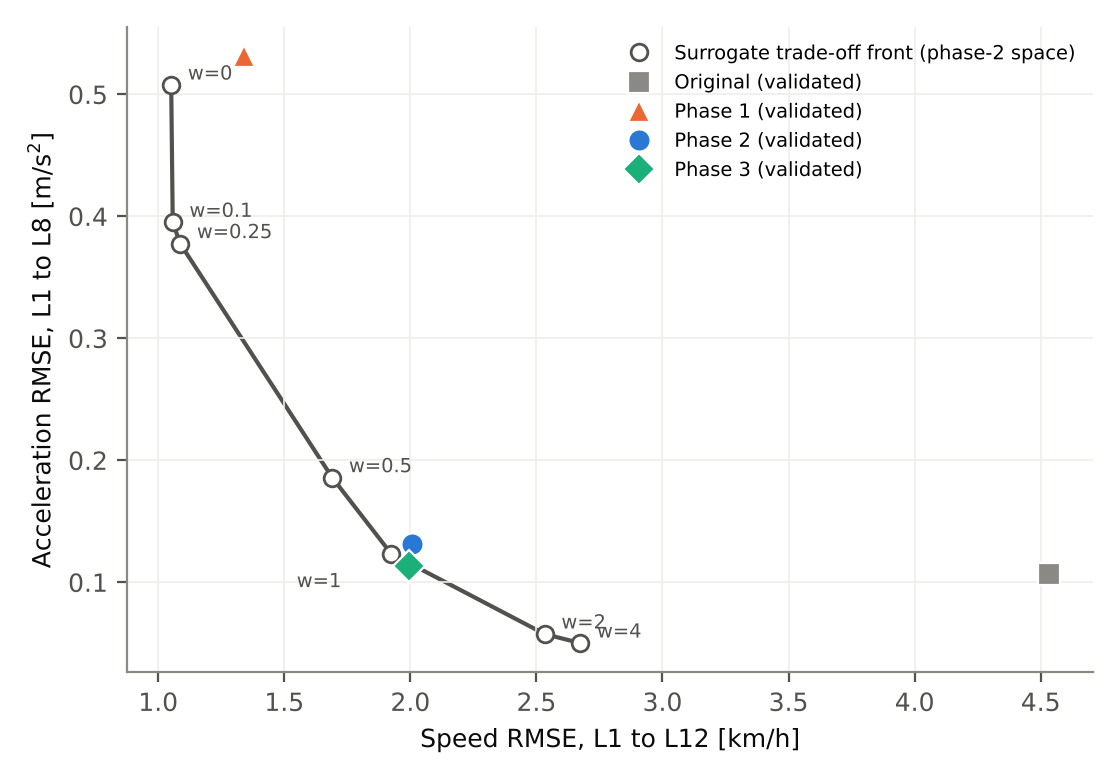
\includegraphics[width=0.72\textwidth]{fig_tradeoff.png}
\caption{Trade-off between speed and acceleration fit. The line connects surrogate optima for
increasing acceleration weight $w$ (phase-2 parameter space); the filled markers are the validated
models with ten independent replications.}
\label{fig:tradeoff}
\end{figure}

%=====================================================================
\section{Phase 3: more freedom and a test-oriented objective}
\label{sec:phase3}
%=====================================================================

\subsection{Changes compared with phase 2}

\begin{enumerate}
  \item \textbf{Objective in units of the $t$-test.} L1 has a field standard deviation of
  4.66~km/h, so a speed error of 3~km/h is statistically acceptable there, whereas at L3
  (0.34~km/h) an error of 0.7~km/h is not. Every error was therefore standardised with the field
  standard deviation of its own location, $z_i = (\bar x_i - \bar y_i)/s_{y,i}$, and penalised by a
  hinge-squared loss that is almost zero inside the acceptance band of the $t$-test and quadratic
  outside it:
  \begin{equation}
  J_3 = \frac{1}{12}\sum_{i=1}^{12} L(z_i^{v}) + \frac{1}{8}\sum_{i=1}^{8} L(z_i^{a}),\qquad
  L(z) = \max(0,|z|-0.75)^2 + 0.05\,z^2 .
  \end{equation}
  With $n_x = n_y = 10$ and similar simulated and field variances the $t$-test passes approximately
  for $|z| < 0.9$, so $J_3$ directly rewards the number of passed tests.
  \item \textbf{Shape of the desired acceleration function.} In the field the vehicles leave the
  junction faster but accelerate less at the exit points than in the model, i.e.\ they accelerate
  harder at low speed and level off earlier. The acceleration function was therefore scaled with
  $\alpha_{\mathrm{lo}}$ up to 20~km/h and $\alpha_{\mathrm{hi}}$ from 50~km/h, linearly
  interpolated in between.
  \item \textbf{Separate right-turn speeds} for vehicles from Kungsgatan (feeding exits L2 and L5)
  and from Slottsgatan (passing L1 and L8).
  \item \textbf{Reuse of all previous simulations.} The 404 configurations of phases 1 and 2 were
  mapped into the phase-3 parameter space (equal values in the new split parameters) and used as
  training data together with 163 new configurations, which reduced the new simulation effort to
  539 runs.
\end{enumerate}

\subsection{Results}

The surrogate trained on 567 configurations reached cross-validated $R^2$ values between 0.976 and
1.00 for the speeds and between 0.91 and 0.99 for the accelerations (Table~\ref{tab:cv}). The
sensitivity map (Figure~\ref{fig:sensitivity}) confirms that the new parameters act where they were
intended: $\alpha_{\mathrm{hi}}$ governs the exit acceleration at L5 ($S_T = 0.70$),
$\alpha_{\mathrm{lo}}$ the exit speeds L5 and L7, the Kungsgatan right-turn speed controls L4
($S_T = 0.76$) and the served flow, and the Slottsgatan right-turn speed controls L8.

The validated phase-3 optimum has practically the same speed RMSE as phase~2 (2.00~km/h), a
slightly lower acceleration RMSE (0.114~m/s$^2$) and a lower test-based objective, but it passes
9 instead of 10 tests. Several of its parameters lie on the boundaries of plausible values
(Slottsgatan right-turn speed 6~km/h, left-turn speed 36~km/h, desired speed Slottsgatan west
58~km/h), which indicates that the optimiser compensates structural limitations of the model rather
than finding better behavioural parameters. Phase~3 therefore confirms that the fit of phase~2 is
close to the best that this model structure allows.

\begin{figure}[H]
\centering
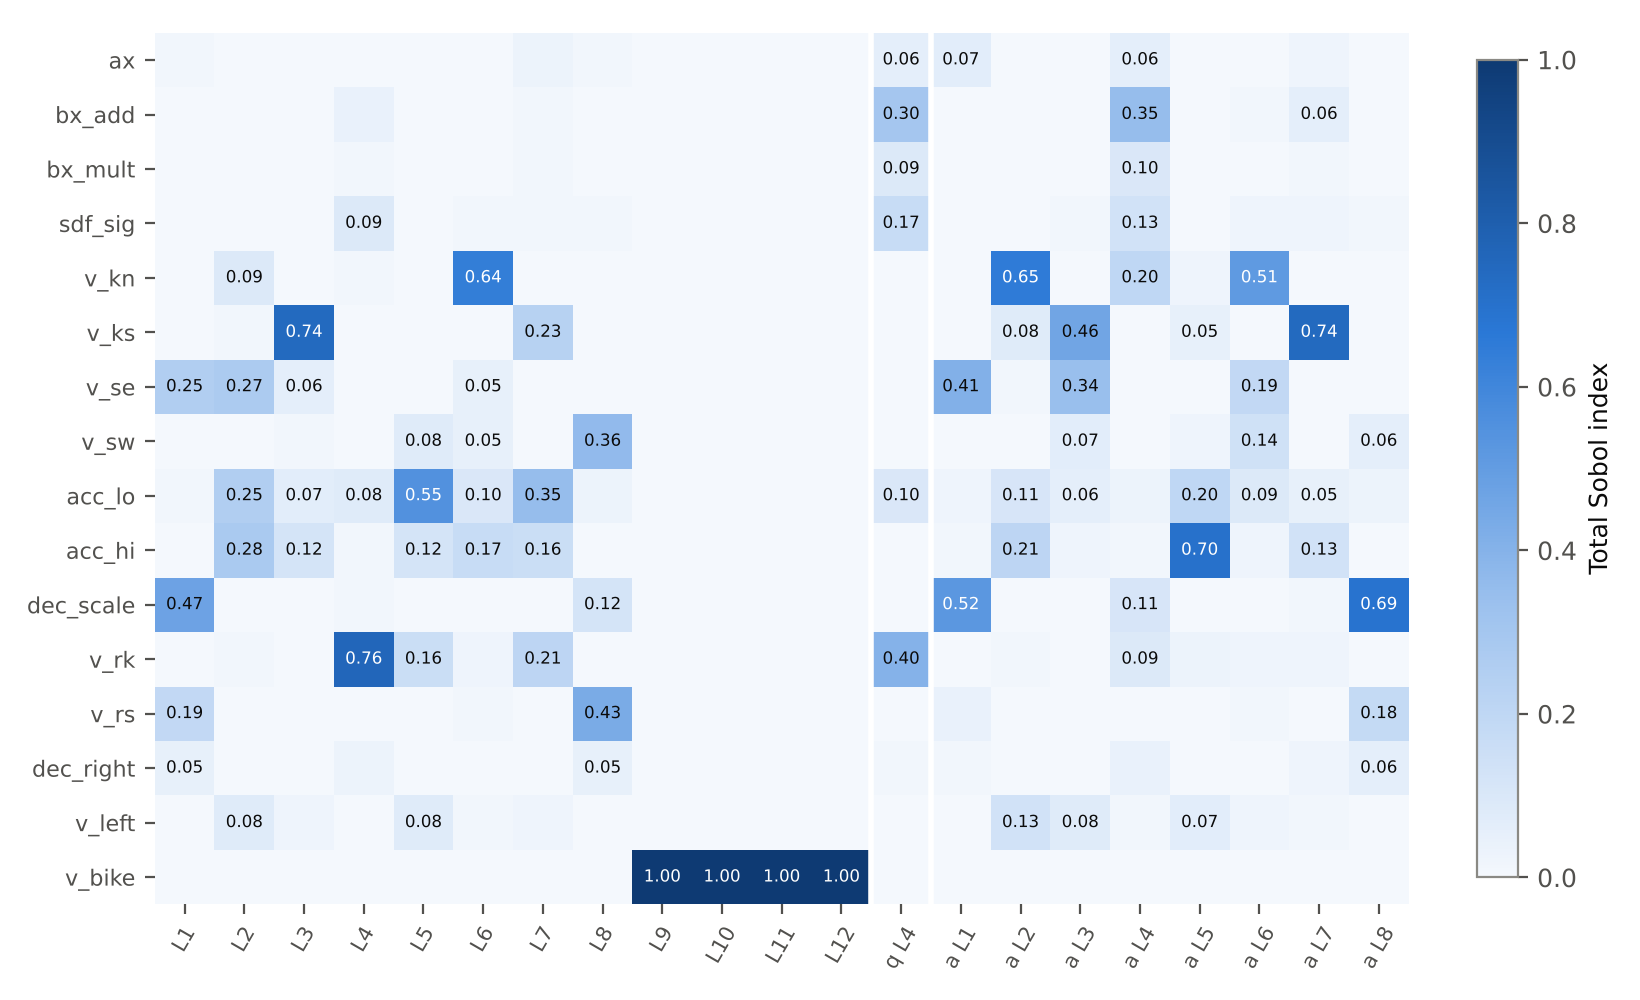
\includegraphics[width=\textwidth]{fig_sensitivity.png}
\caption{Total Sobol indices of the phase-3 parameters for the twelve mean speeds, the served flow
at L4 ($q$ L4) and the eight mean accelerations ($a$ L1 to $a$ L8), estimated on the GP surrogate.
Values below 0.05 are not printed.}
\label{fig:sensitivity}
\end{figure}

\begin{table}[H]
\centering
\caption{Five-fold cross-validated coefficient of determination $R^2$ of the GP surrogates
(phase~3, 567 configurations).}
\label{tab:cv}
\footnotesize
\setlength{\tabcolsep}{3.5pt}
\begin{tabular}{lcccccccccccc}
\toprule
& L1 & L2 & L3 & L4 & L5 & L6 & L7 & L8 & L9 & L10 & L11 & L12\\
\midrule
Speed & 0.995 & 0.997 & 0.996 & 0.976 & 0.997 & 0.992 & 0.986 & 0.993 & 0.999 & 0.998 & 1.000 & 0.998\\
Acceleration & 0.989 & 0.992 & 0.985 & 0.907 & 0.990 & 0.974 & 0.965 & 0.981 & & & & \\
Flow & 0.551 & 0.965 & 0.594 & 0.982 & 0.971 & 0.982 & 0.665 & 1.000 & & & & \\
\bottomrule
\end{tabular}
\end{table}
The low $R^2$ of some flows (L1, L3, L7) is expected: these flows are fixed by the demand and do
not vary with the parameters, so there is almost no variance to explain. The flows that do vary
(L4 and L6, through capacity) are predicted with $R^2 = 0.98$.

%=====================================================================
\section{Validation and comparison of all models}
%=====================================================================

\subsection{Overall comparison}

\begin{table}[H]
\centering
\caption{Validation with ten independent replications (seed 1001, increment 7) against the ten
field mornings. Unfinished vehicles are summed over the ten runs.}
\label{tab:summary}
\small
\begin{tabular}{lrrrr}
\toprule
& \textbf{Original} & \textbf{Phase 1} & \textbf{Phase 2} & \textbf{Phase 3}\\
\midrule
Calibration target & & speeds & speeds + acc. & $t$-test based\\
Speed RMSE, L1 to L12 [km/h] & 4.53 & \textbf{1.34} & 2.01 & 2.00\\
\quad motorised L1 to L8 & 4.85 & 1.64 & 2.46 & 2.44\\
\quad bicycles L9 to L12 & 3.82 & 0.11 & 0.07 & 0.13\\
Acceleration RMSE [m/s$^2$] & \textbf{0.107} & 0.531 & 0.131 & 0.114\\
Speed tests passed & 2/12 & 6/12 & \textbf{7/12} & \textbf{7/12}\\
Acceleration tests passed & \textbf{7/8} & 1/8 & 3/8 & 2/8\\
All tests passed & 9/20 & 7/20 & \textbf{10/20} & 9/20\\
Speed RMSE, odd days / even days & 4.48 / 4.63 & 1.28 / 1.55 & 1.83 / 2.27 & 1.95 / 2.14\\
Maximum GEH, L1 to L8 & 0.68 & 0.68 & 0.68 & 0.69\\
Served flow at L4 [\% of demand] & 100.7 & 99.5 & 101.1 & 101.4\\
Unfinished vehicles (10 runs) & 131 & 224 & 124 & 136\\
\bottomrule
\end{tabular}
\end{table}

All calibrated models serve the demand as well as the original model; the GEH values are far
below 5. The hold-out comparison with the odd and the even field mornings gives nearly the same
RMSE as the comparison with all ten days, so the calibration is not tuned to particular days.

\begin{figure}[H]
\centering
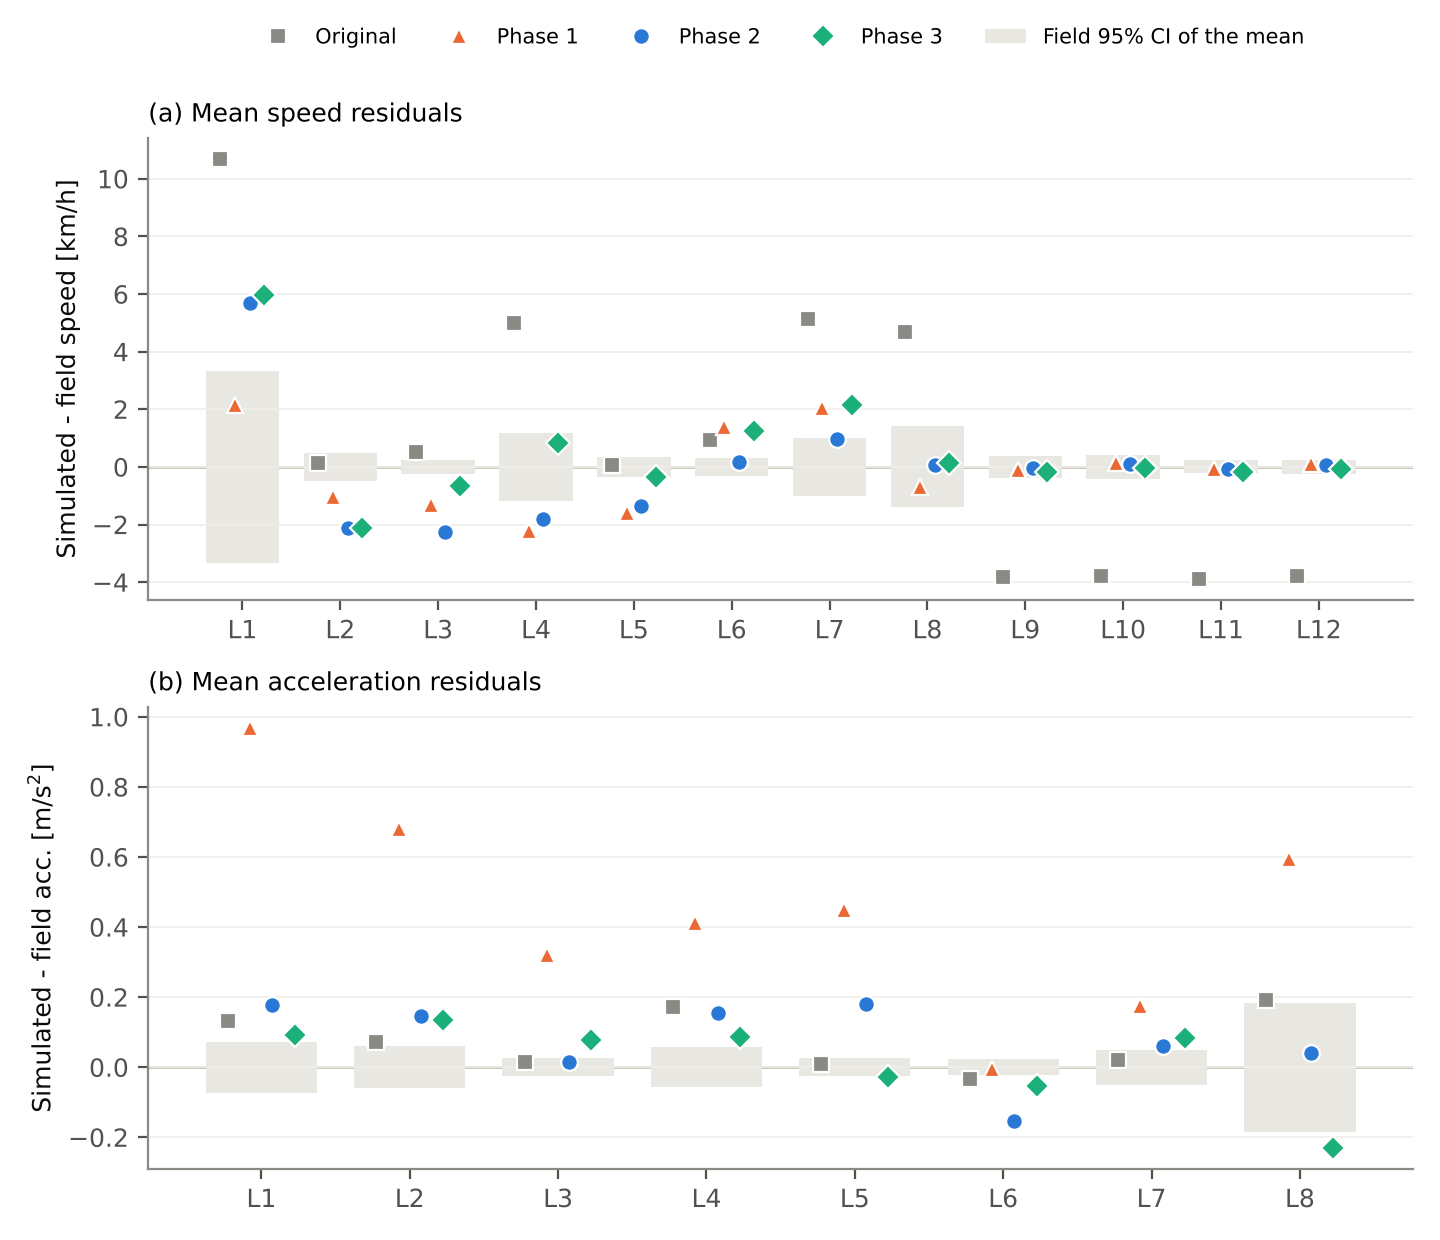
\includegraphics[width=\textwidth]{fig_residuals.png}
\caption{Simulated minus field mean (validation, ten replications) for (a) speeds and (b)
accelerations. The grey bars show the 95\,\% confidence interval of the field mean
($\pm t_{0.975,9}\, s_y/\sqrt{10}$).}
\label{fig:residuals}
\end{figure}

\subsection{Recommended calibrated model}

Phase~2 is recommended as the calibrated model because it passes the most tests, keeps the
acceleration profile of the original model, halves the speed error and has physically plausible
parameter values. Its parameters are given in Table~\ref{tab:calibrated}, together with the
phase-1 and phase-3 solutions for comparison.

\begin{table}[H]
\centering
\caption{Calibrated parameter values. The phase-2 values form the recommended model.}
\label{tab:calibrated}
\small
\begin{tabular}{lrrrr}
\toprule
\textbf{Parameter} & \textbf{Original} & \textbf{Phase 1} & \textbf{Phase 2} & \textbf{Phase 3}\\
\midrule
$a_x$ [m] & 2.00 & 1.83 & 1.49 & 2.05\\
$b_{x,\mathrm{add}}$ & 2.00 & 1.00 & 0.82 & 1.50\\
$b_{x,\mathrm{mult}}$ & 3.00 & 2.00 & 1.39 & 1.18\\
$f_{\mathrm{sig}}$ & 0.60 & 0.55 & 0.31 & 0.34\\
Desired speed Kungsgatan northbound [km/h] & 53.0 & 53.5 & 51.7 & 55.5\\
Desired speed Kungsgatan southbound [km/h] & 53.0 & 53.5 & 51.3 & 55.7\\
Desired speed Slottsgatan east input [km/h] & 53.0 & 53.9 & 43.9 & 44.3\\
Desired speed Slottsgatan west input [km/h] & 53.0 & 53.9 & 52.4 & 58.1\\
Desired acceleration scale & 1.00 & 1.18 & 1.04 & 1.41 / 0.63\\
Desired deceleration scale & 1.00 & 0.50 & 0.89 & 0.94\\
Right-turn speed [km/h] & 22.5 & 13.7 & 10.1 & 11.5 / 6.0\\
Right-turn deceleration [m/s$^2$] & 2.0 & 0.50 & 1.09 & 2.31\\
Left-turn speed [km/h] & (27.5) & 10.0 & 29.9 & 35.7\\
Bicycle / e-bike desired speed [km/h] & 13.5 / 17.5 & 17.6 / 19.9 & 17.3 / 21.3 & 17.2 / 21.2\\
\bottomrule
\end{tabular}

\smallskip
{\footnotesize Phase~3 values given as two numbers: acceleration scale at low / high speed; right-turn
speed from Kungsgatan / Slottsgatan. Phase~1 used one desired speed per street.}
\end{table}

The calibrated values have a clear physical interpretation:
\begin{itemize}
  \item \textbf{Bicycles} need a desired speed of about 17.3~km/h (e-bikes about 21.3~km/h)
  instead of 13.5 and 17.5~km/h. This single change removes the systematic bicycle error of
  3.8~km/h.
  \item \textbf{Right turns} must be considerably slower (about 10~km/h instead of 22.5~km/h). The
  slower right-turners reduce the approach speeds at L1, L4 and L8, where they form 18 to 84\,\% of
  the stream.
  \item \textbf{Slottsgatan east} has a lower desired speed (about 44~km/h) than the other approaches,
  consistent with a narrower urban street and the low approach speed at L1.
  \item \textbf{Car following} becomes slightly tighter ($b_{x,\mathrm{add}}$ and
  $b_{x,\mathrm{mult}}$ lower). This keeps the capacity of the near-saturated northbound approach
  at the demand level even though the slower right-turners would otherwise reduce it.
\end{itemize}

\subsection{Location-wise results of the recommended model}

\begin{table}[H]
\centering
\caption{Mean speeds of the recommended model (phase 2) with ten independent replications
($t_{\mathrm{crit}} = 2.101$). The last column gives $T$ for the original model for comparison.}
\label{tab:locval}
\small
\begin{tabular}{llrrrrrcr}
\toprule
\textbf{Loc.} & \textbf{Name} & \textbf{Field} & \textbf{s.d.} & \textbf{Sim.} & \textbf{s.d.} & $T$ & \textbf{$H_0$ kept} & $T_{\mathrm{orig}}$\\
\midrule
L1  & Slottsgatan East in         & 17.46 & 4.655 & 23.16 & 1.562 &   3.67 & \fail &   6.87\\
L2  & Slottsgatan West out        & 48.71 & 0.688 & 46.58 & 0.426 &  $-8.34$ & \fail &   0.51\\
L3  & Kungsgatan South out        & 49.06 & 0.335 & 46.79 & 0.400 & $-13.72$ & \fail &   3.42\\
L4  & Kungsgatan South in         & 27.00 & 1.629 & 25.20 & 1.155 &  $-2.85$ & \fail &   7.65\\
L5  & Slottsgatan East out        & 40.20 & 0.485 & 38.84 & 0.527 &  $-6.01$ & \fail &   0.32\\
L6  & Kungsgatan North out        & 46.80 & 0.444 & 46.97 & 0.334 &   0.96 & \pass &   4.98\\
L7  & Kungsgatan North in         & 34.41 & 1.414 & 35.37 & 1.383 &   1.53 & \pass &   9.67\\
L8  & Slottsgatan West in         & 19.05 & 1.963 & 19.12 & 1.549 &   0.09 & \pass &   6.21\\
L9  & Kungsgatan South in (bike)  & 18.07 & 0.547 & 18.04 & 0.401 &  $-0.13$ & \pass & $-17.76$\\
L10 & Kungsgatan North out (bike) & 17.70 & 0.574 & 17.81 & 0.435 &   0.47 & \pass & $-16.93$\\
L11 & Kungsgatan North in (bike)  & 18.07 & 0.316 & 18.01 & 0.304 &  $-0.46$ & \pass & $-28.89$\\
L12 & Kungsgatan South out (bike) & 17.77 & 0.331 & 17.83 & 0.339 &   0.38 & \pass & $-25.60$\\
\bottomrule
\end{tabular}
\end{table}

\begin{table}[H]
\centering
\caption{Mean accelerations [m/s$^2$] of the recommended model (phase 2) and of the original model,
ten independent replications.}
\label{tab:accval}
\small
\begin{tabular}{lrrrcrrc}
\toprule
& & \multicolumn{3}{c}{\textbf{Phase 2}} & \multicolumn{3}{c}{\textbf{Original}}\\
\cmidrule(lr){3-5}\cmidrule(lr){6-8}
\textbf{Loc.} & \textbf{Field} & \textbf{Sim.} & $T$ & \textbf{$H_0$ kept} & \textbf{Sim.} & $T$ & \textbf{$H_0$ kept}\\
\midrule
L1 & $-1.787$ & $-1.609$ &  3.12 & \fail & $-1.655$ &  1.63 & \pass\\
L2 &  0.763   &  0.909   &  4.92 & \fail &  0.836   &  1.88 & \pass\\
L3 &  0.505   &  0.519   &  0.78 & \pass &  0.521   &  0.90 & \pass\\
L4 & $-0.214$ & $-0.059$ &  4.65 & \fail & $-0.042$ &  4.51 & \fail\\
L5 &  1.600   &  1.779   &  9.81 & \fail &  1.609   &  0.69 & \pass\\
L6 &  0.724   &  0.572   & $-8.83$ & \fail &  0.690   & $-2.04$ & \pass\\
L7 &  0.966   &  1.028   &  1.88 & \pass &  0.987   &  0.84 & \pass\\
L8 & $-0.710$ & $-0.669$ &  0.46 & \pass & $-0.517$ &  1.83 & \pass\\
\bottomrule
\end{tabular}
\end{table}

The remaining speed failures are of two kinds. At L1 the error of 5.7~km/h is large in absolute
terms but small relative to the day-to-day variation of the field (standard deviation 4.7~km/h);
it fails only because the simulated standard deviation is much smaller. At the exit points L2, L3
and L5 the errors of 1.4 to 2.3~km/h are small in absolute terms but large relative to the very
stable field values (standard deviations 0.3 to 0.7~km/h). The acceleration tests are extremely
strict, because the field standard deviations are only 0.03 to 0.10~m/s$^2$; even the original
model fails at L4.

\subsection{Number of replications}

Table~\ref{tab:repl} gives the number of replications required by the course formula with
$\varepsilon = 0.05$, computed from the ten validation runs.

\begin{table}[H]
\centering
\caption{Required number of replications $n = (t_{0.975,9}\,s_x/(\varepsilon\,\bar x))^2$ for
$\varepsilon = 0.05$, based on the ten validation runs.}
\label{tab:repl}
\footnotesize
\setlength{\tabcolsep}{4pt}
\begin{tabular}{lrrrrrrrrrrrr}
\toprule
& L1 & L2 & L3 & L4 & L5 & L6 & L7 & L8 & L9 & L10 & L11 & L12\\
\midrule
Original & 6.4 & 0.2 & 0.1 & 3.2 & 0.3 & 0.1 & 1.1 & 6.6 & 1.6 & 1.8 & 0.8 & 1.1\\
Phase 2  & 9.3 & 0.2 & 0.1 & 4.3 & 0.4 & 0.1 & 3.1 & 13.4 & 1.0 & 1.2 & 0.6 & 0.7\\
Phase 3  & 12.6 & 0.2 & 0.3 & 3.0 & 0.3 & 0.2 & 4.9 & 17.8 & 1.1 & 1.1 & 0.6 & 0.7\\
\bottomrule
\end{tabular}
\end{table}

The exit points and the cycle tracks need only one or two runs, but the low-speed approach points
L1 and L8, where few vehicles are observed (120 and 90~veh/h) and the speed depends on the signal
phase at arrival, need 10 to 14 runs for the recommended model. Ten replications were used for
validation; for a final evaluation of alternatives 15 replications are recommended. The
calibration runs used three replications with common random numbers. This is sufficient for the
surrogate, because the GP noise term averages the residual simulation noise over hundreds of
configurations, and the validation with independent seeds guards against over-fitting to the
calibration seeds.

%=====================================================================
\section{Alternative designs}
\label{sec:alternatives}
%=====================================================================

\subsection{Scenarios}

The calibrated model (phase~2) was used as the \emph{baseline}: fixed-time controller, program~1,
constant demand, 100 bicycles per hour and direction. All three alternative analyses of the lab
instructions were carried out, each as one modification of the baseline
(Table~\ref{tab:scenarios}). This corresponds to the structure of Vissim's scenario management, in
which every scenario is the base network plus one or more modifications; here the modifications
were applied by the same Python tool chain that was used for the calibration, so that every
scenario is generated from exactly the same calibrated network.

\begin{table}[H]
\centering
\caption{Simulated scenarios. All other settings are identical to the calibrated baseline.}
\label{tab:scenarios}
\small
\begin{tabularx}{\textwidth}{lX}
\toprule
\textbf{Scenario} & \textbf{Modification of the baseline}\\
\midrule
Baseline & Calibrated model (phase~2), fixed-time controller, program~1 (cycle 90~s), constant demand.\\
Actuated control & Signal controller switched to type VAP with the provided logic
\texttt{Control\_logic.vap} and the interstage file \texttt{Signal\_data.pua}. Stage~1 (Kungsgatan)
is extended while a vehicle is detected within a gap of 3~s on detectors 1, 2, 4 or 5, up to a
stage time of 75~s; stage~2 (Slottsgatan) is called by detectors 3 or 6 and extended in the same way
up to 15~s.\\
Incident demand & Vehicle inputs A (Kungsgatan north), C (Slottsgatan east), E (Kungsgatan south)
and G (Slottsgatan west) change every 10 minutes according to Table~1 of the lab instructions
(A: 670, 640, 670; C: 160, 370, 190; E: 1100, 920, 1100; G: 100, 380, 150~veh/h). The warm-up uses
the baseline demand.\\
800 bicycles/h & Bicycle demand increased from 100 to 800 bicycles per hour in each direction,
constant over the period.\\
\bottomrule
\end{tabularx}
\end{table}

Note that the 30-minute averages of the incident demand are exactly equal to the baseline demand
(660, 240, 1040 and 210~veh/h). The incident scenario therefore tests the effect of the
\emph{temporal} redistribution of the demand, not of additional traffic.

\subsection{Experimental setup and traffic metrics}

Each scenario was simulated with 20 replications and the same random seeds as the baseline (seed
42, increment 1), 600~s warm-up and 1\,800~s of evaluation. With common random numbers, replication
$k$ of a scenario sees the same random arrivals as replication $k$ of the baseline, so differences
were tested with a paired $t$-test on the 20 replication-wise differences. The required number of
replications for the average delay (course formula, $\varepsilon = 5\,\%$) is 12 for the baseline,
16 for the actuated controller, 10 for the incident and 6 for the bicycle scenario, so 20
replications are sufficient.

The following metrics were chosen:
\begin{itemize}
  \item \textbf{Average delay per vehicle} (vehicle network performance): the standard measure of
  the level of service of a signalised intersection, and the quantity a signal control strategy
  aims to reduce.
  \item \textbf{Stops per vehicle} and \textbf{stopped delay}: indicators of driving comfort,
  emissions and the number of acceleration manoeuvres.
  \item \textbf{Mean and maximum queue length} at the ten queue counters (main lanes, left-turn
  pockets and both cycle tracks), in 10-minute intervals: queues show \emph{where} the delay
  occurs, whether the storage space is sufficient, and how a temporary demand change builds up and
  dissolves.
  \item \textbf{Speeds and flows} at the twelve measurement locations: they connect the scenarios
  to the calibration and show the effect on the bicycle tracks and on the throughput.
\end{itemize}

\subsection{Results}

\begin{table}[H]
\centering
\caption{Vehicle network performance, all vehicles (mean $\pm$ 95\,\% confidence half-width,
20 replications). $\Delta$: paired difference to the baseline; $p$: paired $t$-test.}
\label{tab:altperf}
\footnotesize
\setlength{\tabcolsep}{4pt}
\begin{tabular}{lrrrrrr}
\toprule
\textbf{Scenario} & \textbf{Delay [s/veh]} & $\Delta$ & $p$ & \textbf{Stops [1/veh]} & \textbf{Speed [km/h]} & \textbf{Arrived [veh]}\\
\midrule
Baseline         & $21.3 \pm 0.8$ &        &          & $0.74$ & $13.2$ & 1\,264\\
Actuated control & $15.7 \pm 0.7$ & $-5.6$ & $<0.001$ & $0.66$ & $15.9$ & 1\,265\\
Incident demand  & $21.3 \pm 0.8$ & $+0.1$ & 0.67     & $0.75$ & $13.1$ & 1\,262\\
800 bicycles/h   & $22.5 \pm 0.6$ & $+1.2$ & $<0.001$ & $1.51$ & $11.3$ & 1\,917\\
\bottomrule
\end{tabular}
\end{table}

\begin{figure}[H]
\centering
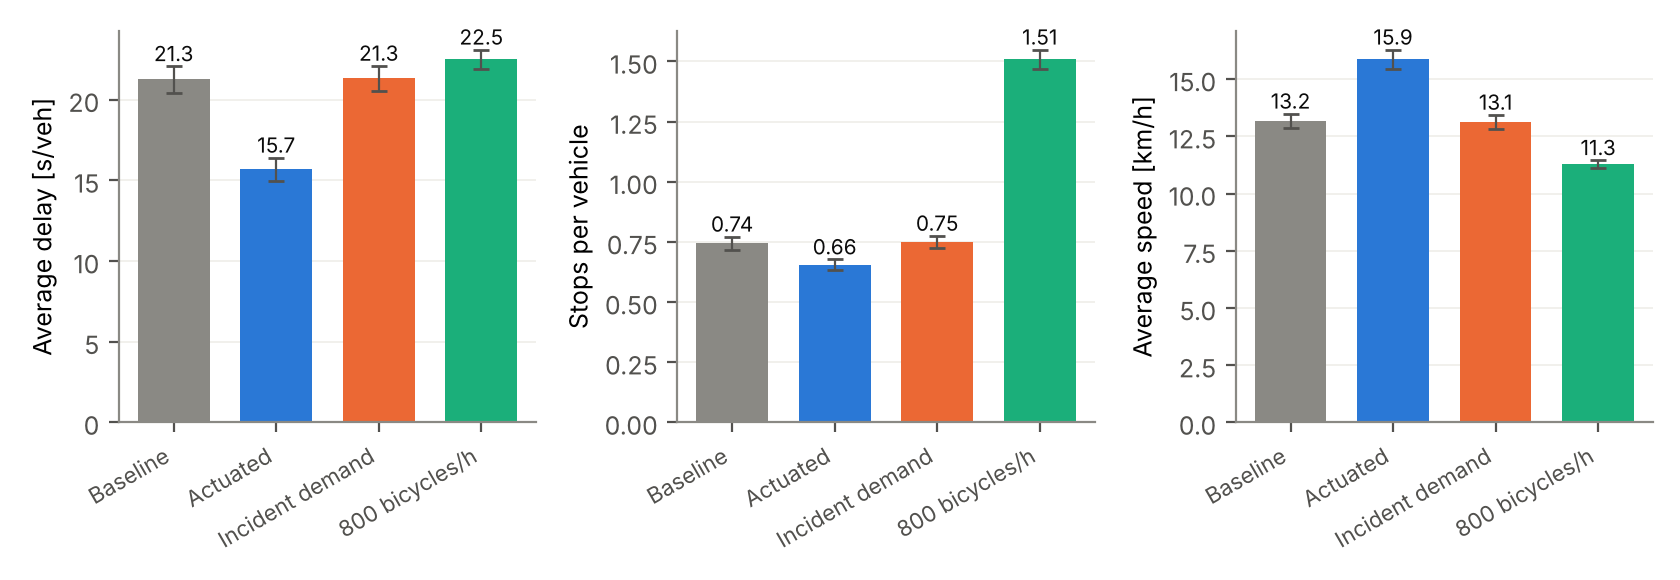
\includegraphics[width=\textwidth]{fig_alt_network.png}
\caption{Average delay, stops and speed of all vehicles (mean and 95\,\% confidence interval,
20 replications).}
\label{fig:altnet}
\end{figure}

\begin{figure}[H]
\centering
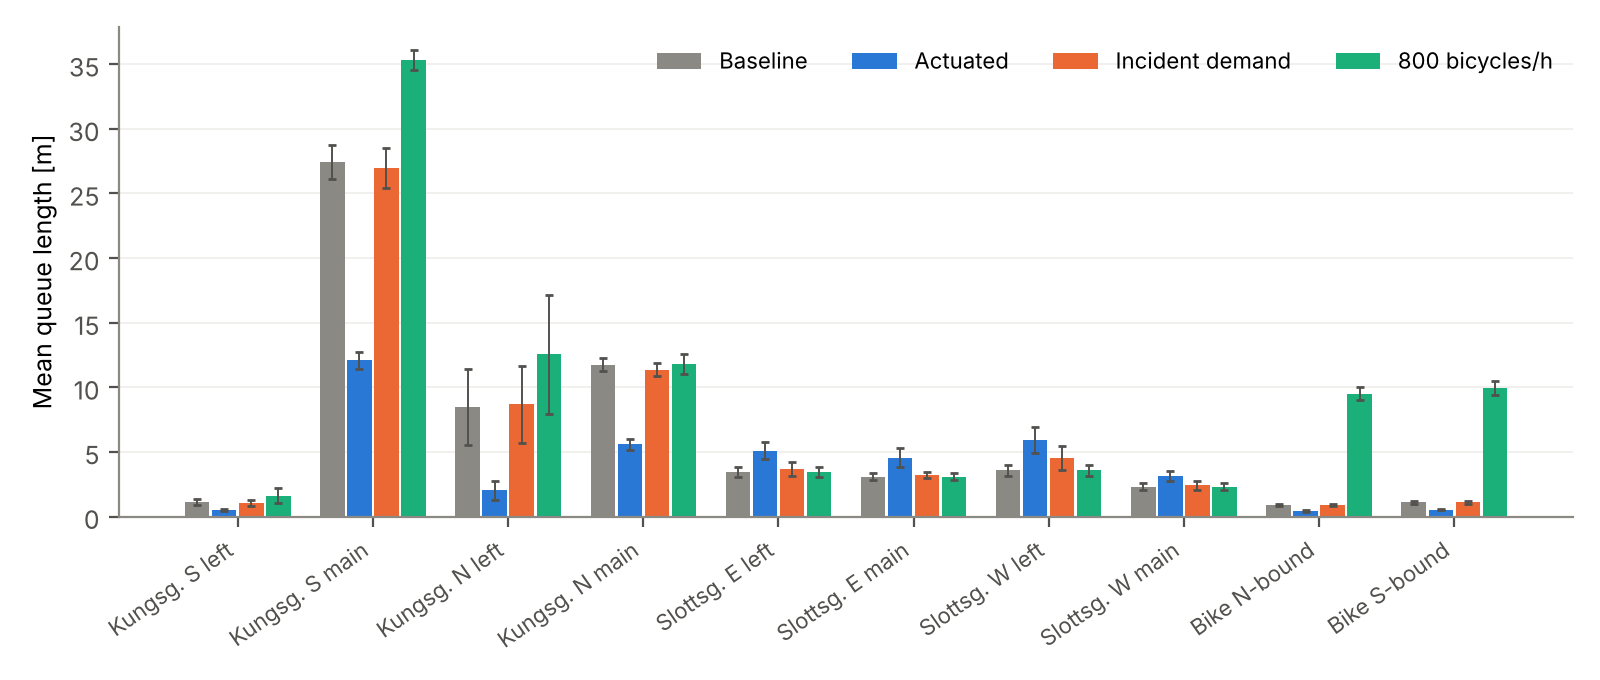
\includegraphics[width=\textwidth]{fig_alt_queue.png}
\caption{Mean queue length per queue counter over the 30-minute evaluation period (mean and
95\,\% confidence interval, 20 replications).}
\label{fig:altqueue}
\end{figure}

\paragraph{Actuated signal control.} The actuated controller reduces the average delay of all
vehicles by 5.6~s, from 21.3 to 15.7~s per vehicle ($-26\,\%$, $p < 0.001$), the number of stops by
12\,\% and the stopped delay from 13.9 to 9.0~s. The improvement comes from Kungsgatan: the mean
queue on the critical northbound lane falls from 27.5 to 12.1~m and the southbound queue from 11.8
to 5.6~m, while the Slottsgatan queues grow by 1 to 2~m. The fixed-time plan gives Slottsgatan 38~s
of green although it carries only about 20\,\% of the traffic; the actuated logic ends the
Slottsgatan stage as soon as the gaps exceed 3~s and gives the time to the heavily loaded main
road. The price is paid by the minor road: the approach speeds at L1 and L8 decrease (from 23.6 to
21.7 and from 19.2 to 16.8~km/h) because more Slottsgatan vehicles arrive on red. The cyclists on
Kungsgatan, who share stage~1, also benefit (bicycle queues halved). The total throughput is
unchanged.

\paragraph{Incident with variable demand.} Over the whole 30 minutes the incident scenario does not
differ from the baseline (delay $+0.1$~s, $p = 0.67$), which is expected because the average demand
is identical. The temporal analysis (Figure~\ref{fig:altincident}) shows the effect of the
incident: in the second interval, when the Slottsgatan demand increases to 370 and 380~veh/h,
the left-turn queues on Slottsgatan double (east, from 3.2 to 6.6~m) and almost triple (west, from
3.6 to 9.6~m). At the same time the reduced Kungsgatan demand (920 instead of 1100~veh/h northbound)
shortens the northbound queue slightly. In the third interval all queues return to the baseline
level. The fixed-time plan therefore has enough reserve capacity on Slottsgatan to absorb the
10-minute peak without residual queues; the critical approach remains Kungsgatan northbound,
whose demand of 1100~veh/h in the first and last interval is close to its capacity in both
scenarios.

\begin{figure}[H]
\centering
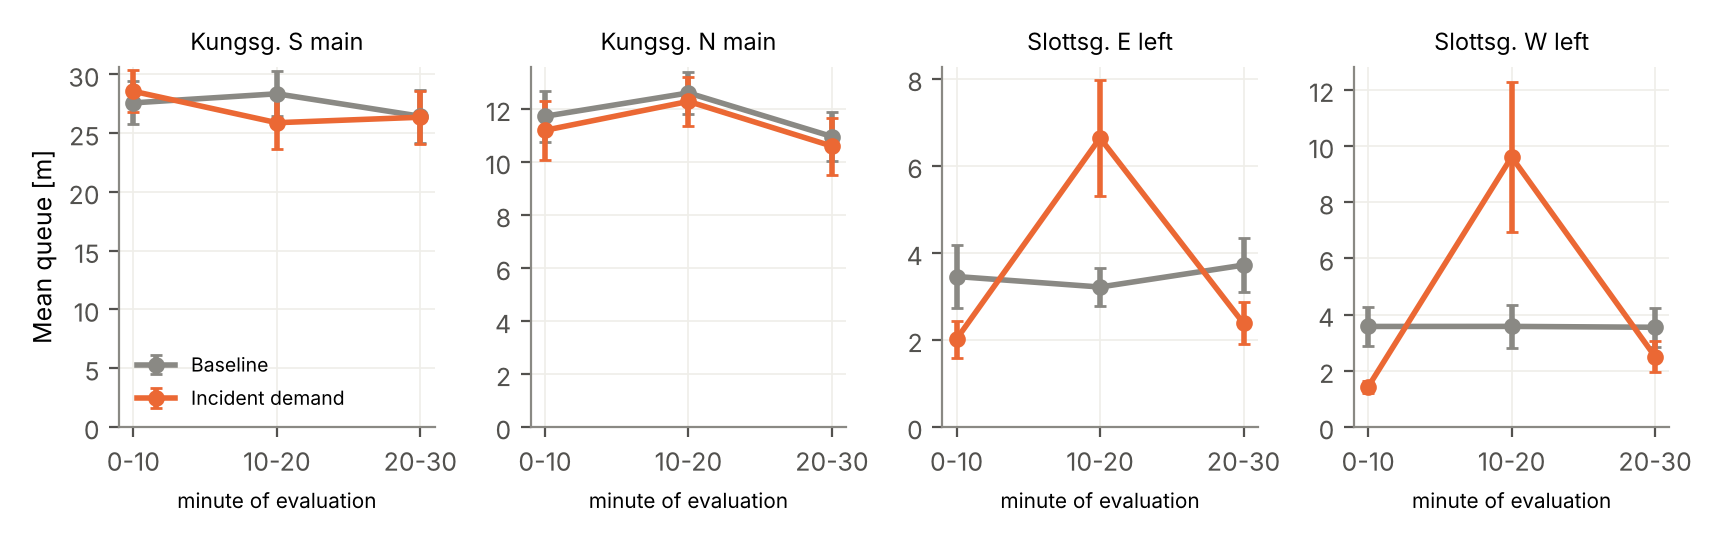
\includegraphics[width=\textwidth]{fig_alt_incident.png}
\caption{Mean queue length per 10-minute interval for the baseline and the incident demand
(mean and 95\,\% confidence interval, 20 replications).}
\label{fig:altincident}
\end{figure}

\paragraph{Increase of bicycle demand to 800 per direction.} The eightfold bicycle demand has two
effects. For the cyclists themselves, the mean speed on the cycle tracks decreases from 17.9 to
16.5~km/h (up to $-2.1$~km/h at the points before the bicycle stop lines, L9 and L11) and the
bicycle queues at the stop lines grow from about 1 to 10~m (maximum 57~m). For motorised traffic,
the right-turning vehicles from Kungsgatan must yield to a nearly continuous stream of cyclists.
The flow that passes L4 and L6 drops from 943 to 878~veh/h and from 999 to 945~veh/h ($-7\,\%$);
the northbound queue grows from 27.5 to 35.3~m and the southbound left-turn queue from 8.5 to
12.6~m. The number of stops per vehicle doubles (0.74 to 1.51, mainly bicycle stops at red), and
the average delay rises by 1.2~s per vehicle. This average underestimates the effect on cars,
because the many bicycles with moderate delay enter the average and because the vehicles that can
no longer enter the network on Kungsgatan are not counted. The bicycle scenario thus shows that
the conflict between right-turning cars and cyclists, not the bicycle signal itself, is the
capacity bottleneck at higher bicycle volumes.

\begin{table}[H]
\centering
\caption{Mean speed [km/h] and hourly flow [veh/h] at selected measurement locations.}
\label{tab:altloc}
\small
\begin{tabular}{llrrrr}
\toprule
\textbf{Loc.} & \textbf{Quantity} & \textbf{Baseline} & \textbf{Actuated} & \textbf{Incident} & \textbf{800 bicycles/h}\\
\midrule
L1 & speed & 23.6 & 21.7 & 23.2 & 23.6\\
L4 & speed & 25.7 & 27.1 & 25.8 & 25.4\\
L4 & flow  & 943  & 947  & 937  & 878\\
L6 & flow  & 999  & 1\,002 & 995 & 945\\
L7 & speed & 35.9 & 36.4 & 36.3 & 35.9\\
L8 & speed & 19.2 & 16.8 & 18.9 & 19.2\\
L9 to L12 & bicycle speed & 17.9 & 18.0 & 17.9 & 16.5\\
\bottomrule
\end{tabular}
\end{table}

\subsection{Comparison of the alternatives}

\begin{itemize}
  \item The actuated controller is the only alternative that improves the intersection, and the
  improvement is large and statistically clear. It mainly reallocates green time from the lightly
  loaded side road to the near-saturated main road; the side road and its right-turners wait
  somewhat longer.
  \item A short-term redistribution of demand of the size in Table~1 is absorbed by the
  fixed-time plan; it causes temporary queues on Slottsgatan but no lasting degradation. Measures
  aggregated over 30 minutes hide this effect completely, which shows why time-resolved metrics are
  needed for incident analyses.
  \item A strong increase of cycling reduces the car capacity on Kungsgatan by about 7\,\% through
  the right-turn conflicts and doubles the number of stops, while the cycling speeds fall only
  moderately. Measures such as a separate right-turn phase or a leading bicycle interval would be
  natural next steps to analyse.
\end{itemize}

%=====================================================================
\section{Discussion}
%=====================================================================

\paragraph{Value of the surrogate approach.} About 1\,860 runs were sufficient to map a
14- to 16-dimensional parameter space with a predictive accuracy of $R^2 \ge 0.97$ for all speeds.
The surrogate made it possible to compute global sensitivity indices, to optimise under constraints
in seconds, to explore the trade-off between conflicting targets and to reuse all earlier runs
when the parameterisation was extended. A one-at-a-time search would not have revealed the
interaction between car following, right-turn speed and capacity at L4, nor the fact that the
speed-only optimum relies on unrealistic deceleration.

\paragraph{Choice of the calibration target.} The three phases show that the result depends at least
as much on the objective as on the parameters. Fitting speeds alone gives the lowest speed RMSE
but an invalid model. Adding accelerations restores the dynamics. Weighting each location by its
own field variability corresponds to the statistical test used for acceptance but cannot overcome
structural conflicts. A calibration report should therefore always state the objective and show
more than one performance measure.

\paragraph{Structural limitations.} Two conflicts remain in every phase: the approach at L1
(low speed together with strong deceleration) and the exits, which are slightly too slow while
the model already accelerates harder than observed. Both point to the representation of turning
movements (reduced-speed areas only on the connectors, after the stop line) and to the use of one
desired acceleration function for all situations. Possible improvements outside the scope of
parameter calibration are reduced-speed areas or desired speed decisions upstream of the stop
lines, separate vehicle types or driving behaviours for turning traffic, and a check of the
detector positions in the network against the field measurement positions.

\paragraph{Demand constraint.} Without the served-demand constraint the optimiser preferred
configurations in which up to 30\,\% of the northbound demand could not enter the network, because
the resulting congestion lowers the speed at L4. Checking GEH and unfinished vehicle inputs is
therefore an essential part of the calibration and not only of the validation.

\paragraph{Alternatives.} The scenario results are only as reliable as the calibrated model in
the situations it was calibrated for. The actuated controller and the incident change the timing and
the demand, which the calibration covers well. The bicycle scenario relies on the interaction
between cyclists and right-turning cars at the conflict areas, whose parameters could not be
calibrated because they had no influence on the measured speeds at 100 bicycles per hour; this
result should therefore be regarded as more uncertain.

\paragraph{Limitations.} The field data provide no flow counts, so the demand of the model was
taken as correct. The surrogate optimum is only as good as the surrogate; this was controlled by
cross-validation and by validating several distinct optima with independent seeds. The bicycle
speeds identify only the flow-weighted mean desired speed of bicycles and e-bikes; the split
between the two types was fixed.

%=====================================================================
\section{Conclusions}
%=====================================================================

\begin{itemize}
  \item A fully automated calibration chain (model variant generation, Vissim COM control, result
  extraction, GP surrogates, sensitivity analysis, constrained optimisation and validation) was
  developed and applied in three phases with about 1\,860 simulation runs.
  \item The original model deviates mainly at the approaches (L1, L4, L7, L8) and on the cycle
  tracks; with warm-up it passes 2 of 12 speed tests and has a speed RMSE of 4.53~km/h.
  \item The most influential parameters are the right-turn speed, the Slottsgatan and Kungsgatan
  desired speeds, the desired acceleration and deceleration functions and the bicycle desired speed;
  the conflict-area gap parameters have no influence.
  \item Calibrating on speeds only (phase~1) produces an invalid model with unrealistic dynamics.
  \item The recommended model (phase~2) halves the speed RMSE to 2.01~km/h, keeps the acceleration
  RMSE at 0.13~m/s$^2$, passes 10 of 20 tests including all bicycle locations, serves the demand
  (GEH $\le 0.68$) and is stable on independent seeds and on odd and even field days.
  \item The remaining discrepancies are structural; additional parameter freedom (phase~3) does not
  improve the test results further.
  \item The approach points require 10 to 14 replications for a relative error of 5\,\%; 15
  replications are recommended for the analysis of alternative designs.
  \item Alternative designs (20 paired replications): the actuated controller reduces the average
  delay by 5.6~s per vehicle ($-26\,\%$) and the main-road queues by more than half; the incident
  demand causes only temporary side-road queues; 800 bicycles per direction reduce the car
  throughput on Kungsgatan by 7\,\% and double the stops.
\end{itemize}

%=====================================================================
\section{Reflections}
%=====================================================================

The exercise illustrates several general points about microscopic traffic simulation. First, a
simulation model is a hypothesis about behaviour, and calibration tests this hypothesis against
data; the phases above show that a good fit of one indicator (speeds) can hide a wrong mechanism
(braking behaviour), so that several independent indicators are needed. Second, the stochastic
nature of the model must be handled explicitly: warm-up, the number of replications, common random
numbers for comparisons and independent seeds for validation all changed the conclusions noticeably.
Third, treating the simulator as an expensive black-box function and replacing it by a statistical
surrogate turns calibration into a well-defined optimisation and sensitivity problem, which makes
the process transparent and reproducible, but the choice of the objective remains an engineering
decision that has to be justified. Finally, the alternative designs show that the value of a
calibrated model lies in comparing alternatives under identical conditions: the absolute numbers
carry the remaining calibration error, but the paired differences between scenarios are precise and
robust.
% Add here the links to the topics of the previous seminars of the course.

%=====================================================================
\appendix
\section{Reproducibility}
%=====================================================================

All scripts, designs, raw results (one row per configuration, replication and location),
training and validation reports are stored next to the model in the folders
\texttt{Calibration}, \texttt{Calibration\_phase2} and \texttt{Calibration\_phase3}. A complete
phase is reproduced on the Vissim computer with the commands below; the alternative designs are in
the folder \texttt{Alternatives} (\texttt{py run\_alternatives.py all}).
\begin{verbatim}
py run_pipeline.py smoke      # COM check, 2 configurations x 1 run
py run_pipeline.py all        # screening, refinement, validation
\end{verbatim}
Table~\ref{tab:effort} summarises the simulation effort.

\begin{table}[H]
\centering
\caption{Simulation effort (one run = 2\,400~s of simulated time).}
\label{tab:effort}
\small
\begin{tabular}{lrrrr}
\toprule
& \textbf{Screening} & \textbf{Refinement} & \textbf{Validation} & \textbf{Runs}\\
\midrule
Phase 1 & $162 \times 3$ & $41 \times 3$ & $5 \times 10$ & 659\\
Phase 2 & $162 \times 3$ & $41 \times 3$ & $5 \times 10$ & 659\\
Phase 3 & $122 \times 3$ & $41 \times 3$ & $5 \times 10$ & 539\\
Alternatives & & & $4 \times 20$ & 80\\
\midrule
Total & & & & 1\,937\\
\bottomrule
\end{tabular}
\end{table}

\end{document}
